% !TEX root = ../main.tex
%---------------------------------------------------------------------------------------------------
\section*{Urn example}
%---------------------------------------------------------------------------------------------------
We now illustrate the key ideas of evaluating statistical decision functions with an urn example. We study a set of decision functions and first compare the performance of two distinct rules before determining the optimal rule within the whole set.\\

We consider an urn with black $b$ and white $w$ balls where the true proportion of black balls $\theta_0$ is unknown. In this example, the action constitutes a guess $\tilde{\theta}$ about $\theta_0$ after drawing a fixed number of $n$ balls at random with replacement. The parameter and action space both correspond to the unit interval $\Theta = \A = [0, 1]$. \\

If the guess matches the true proportion, we receive a payment of one. On the other hand, in case of a discrepancy, the payment is reduced by the squared error. Thus, the consequence function takes the following form:
%
\begin{align*}
\rho(\tilde{\theta}, \theta_0) = 1 - (\tilde{\theta} - \theta_0)^2.
\end{align*}
%
The sample space is $\Psi = \{b, w\}^n$ where a sequence $(b, w, b, \hdots, b)$ of length $n$ is a typical realization of $\psi$. The observed number of black balls $r$ among the $n$ draws in a given sample $\psi$ provides a signal about $\theta_0$. The sampling distribution for the possible number of black balls $R$ takes the form of a probability mass function (PMF):
%
\begin{align*}
\Pr(R = r) = \left(\begin{array}{c} n \\ r \end{array} \right)\, (\theta_0)^r\, (1 - \theta_0)^{n-r}.
\end{align*}
%
Any function $\delta:  \{b, w\}^n \mapsto [0, 1]$ that maps the number of black draws to the unit interval is a possible statistical decision function.\\

For an illustration of our methods, we focus on the following class of decision functions $\delta \in \Gamma$:
%
\begin{align*}
 \delta(r, \lambda) = \lambda\,\left(\frac{r}{n}\right)  + (1 - \lambda)\,\left(\frac{1}{2}\right),\qquad\text{for some}\quad 0 \leq \lambda \leq 1.
\end{align*}
%
The empirical proportion of black balls in the sample $r / n$ provides the point estimate $\hat{\theta}$. The decision function specifies the guess as a weighted average between the point estimate itself and the midpoint of the parameter space. The larger $\lambda$, the more weight is put on the point estimate. Each $\lambda$ indexes a particular decision function. At the extremes, at $\lambda = 1$, the guess is the point estimate, while for $\lambda = 0$, the guess is fixed at $0.5$.\\

We later determine the best decision function within this class, but we start by comparing the performance of the two decision functions with $\lambda = 1$ and $\lambda = 0.9$. We refer to the former as the as-if decision function as it announces the point estimate as-if it is the true one and $\lambda=0.9$ as the robust decision function for reasons that will become clear later. We evaluate their relative performance by aggregating the vector of expected payoffs over the unit interval using the different decision-theoretic criteria. We assume a linear utility function and thus directly refer to the monetary consequences of a guess as its payoff. Throughout, we set the number of draws $n$ to  $50$.\\

Figure \ref{Calculation of expected payoff} shows the sampling distribution of the number of black balls $R$, the associated payoff for each possible draw, and the two decision functions. The true but unknown share in this example is $40\%$, i.e. $\theta = 0.4$. The robust decision function outperforms the as-if rule for realizations of the point estimate smaller than its true value due to the shift towards $0.5$. At the same time, the as-if rule leads to a higher payoff at the center of the distribution.\\

\begin{figure}[h!]\centering
\scalebox{0.75}{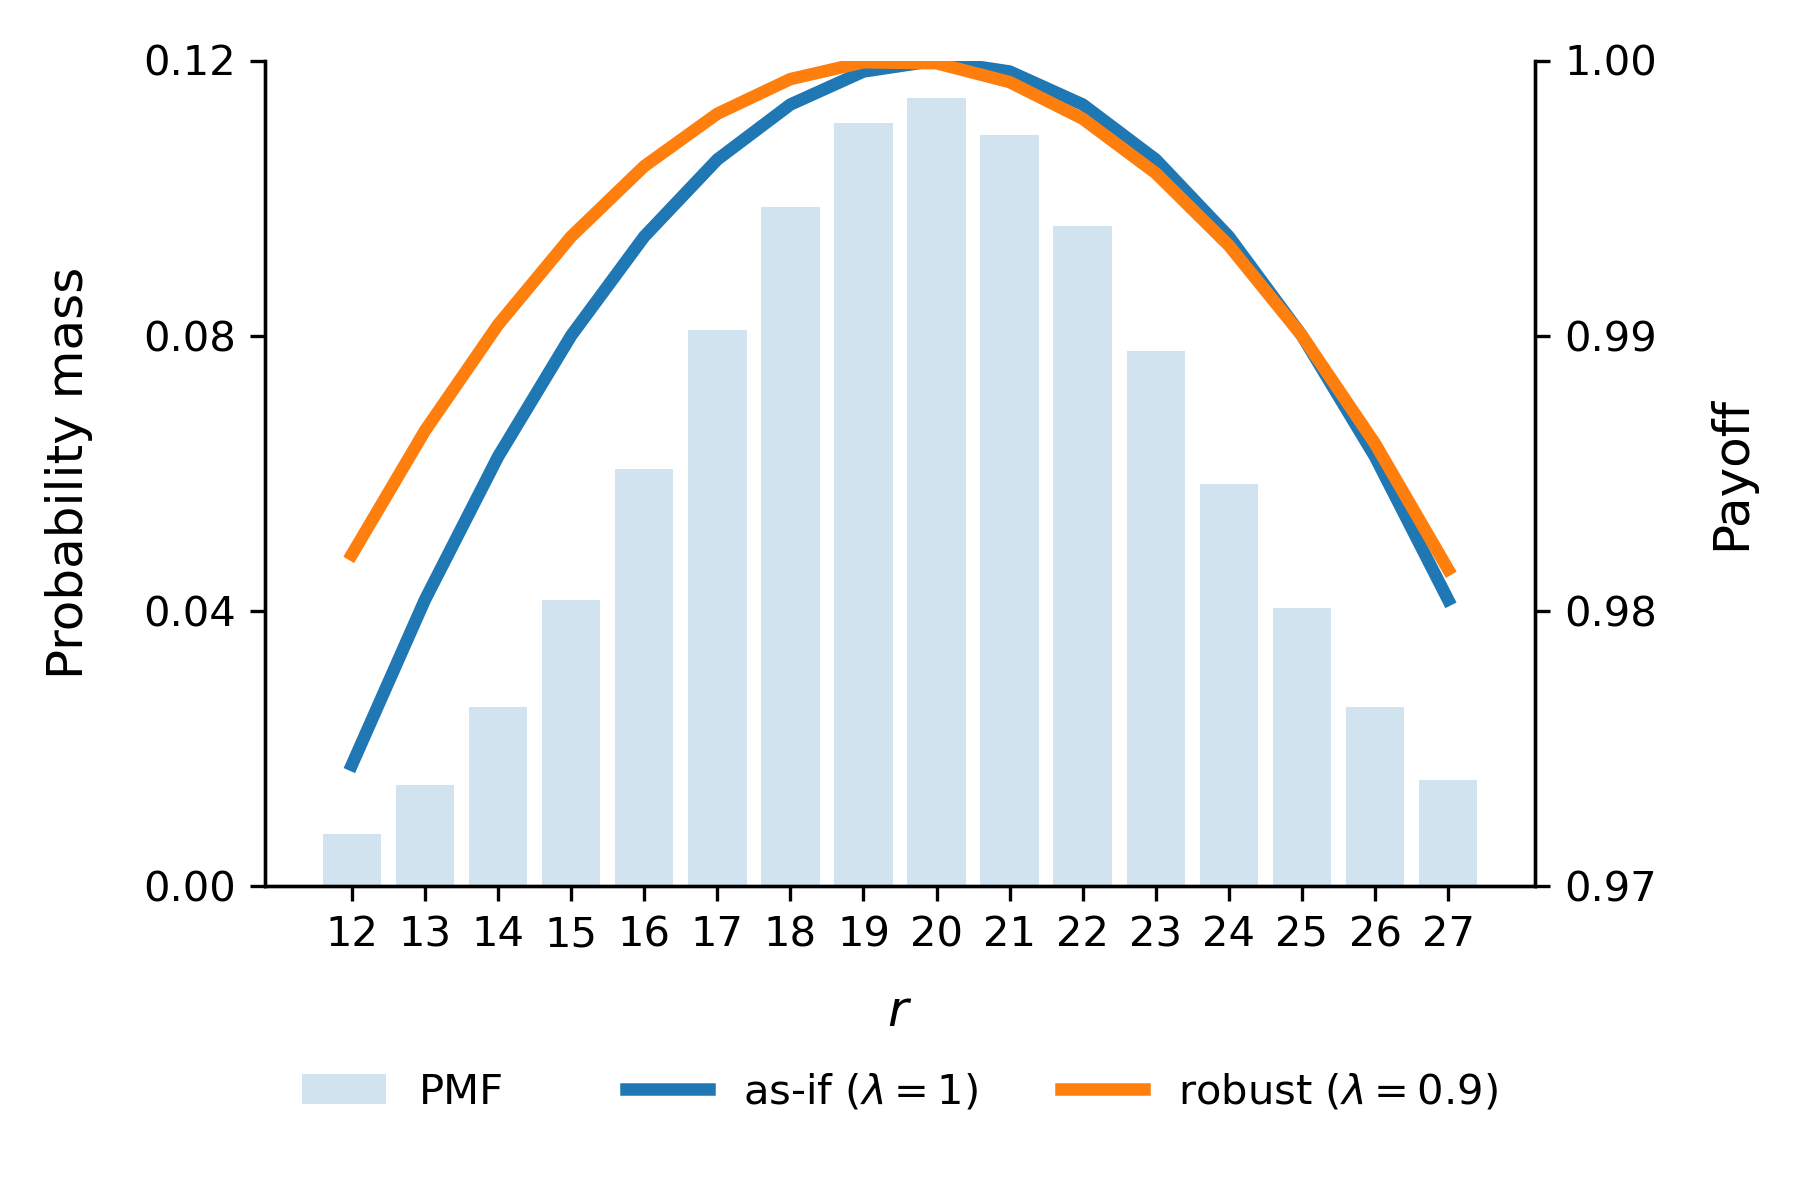
\includegraphics{fig-example-urn-expected-payoff}}
\caption{Calculating the expected payoff}\label{Calculation of expected payoff}
\end{figure}\FloatBarrier

Figure \ref{Measurement of performance} shows the expected payoff at different points in the parameter space. On the left, we show the expected payoff at two selected points. While the as-if decision function performs better than the robust rule at $\theta = 0.1$, the opposite is true at $\theta = 0.4$. Thus, both decision functions are admissible as neither of the two outperforms the other for all possible true proportions. On the right, we trace out the expected payoff of both rules over the whole parameter space. The robust rule outperforms the as-if rule in the center of the parameter space but performs worse at the boundary. Overall, the performance of the robust rule is more balanced across the whole parameter space, which motivates its name.

\begin{figure}[h!]\centering
\subfloat[Expected payoff]{\scalebox{0.50}{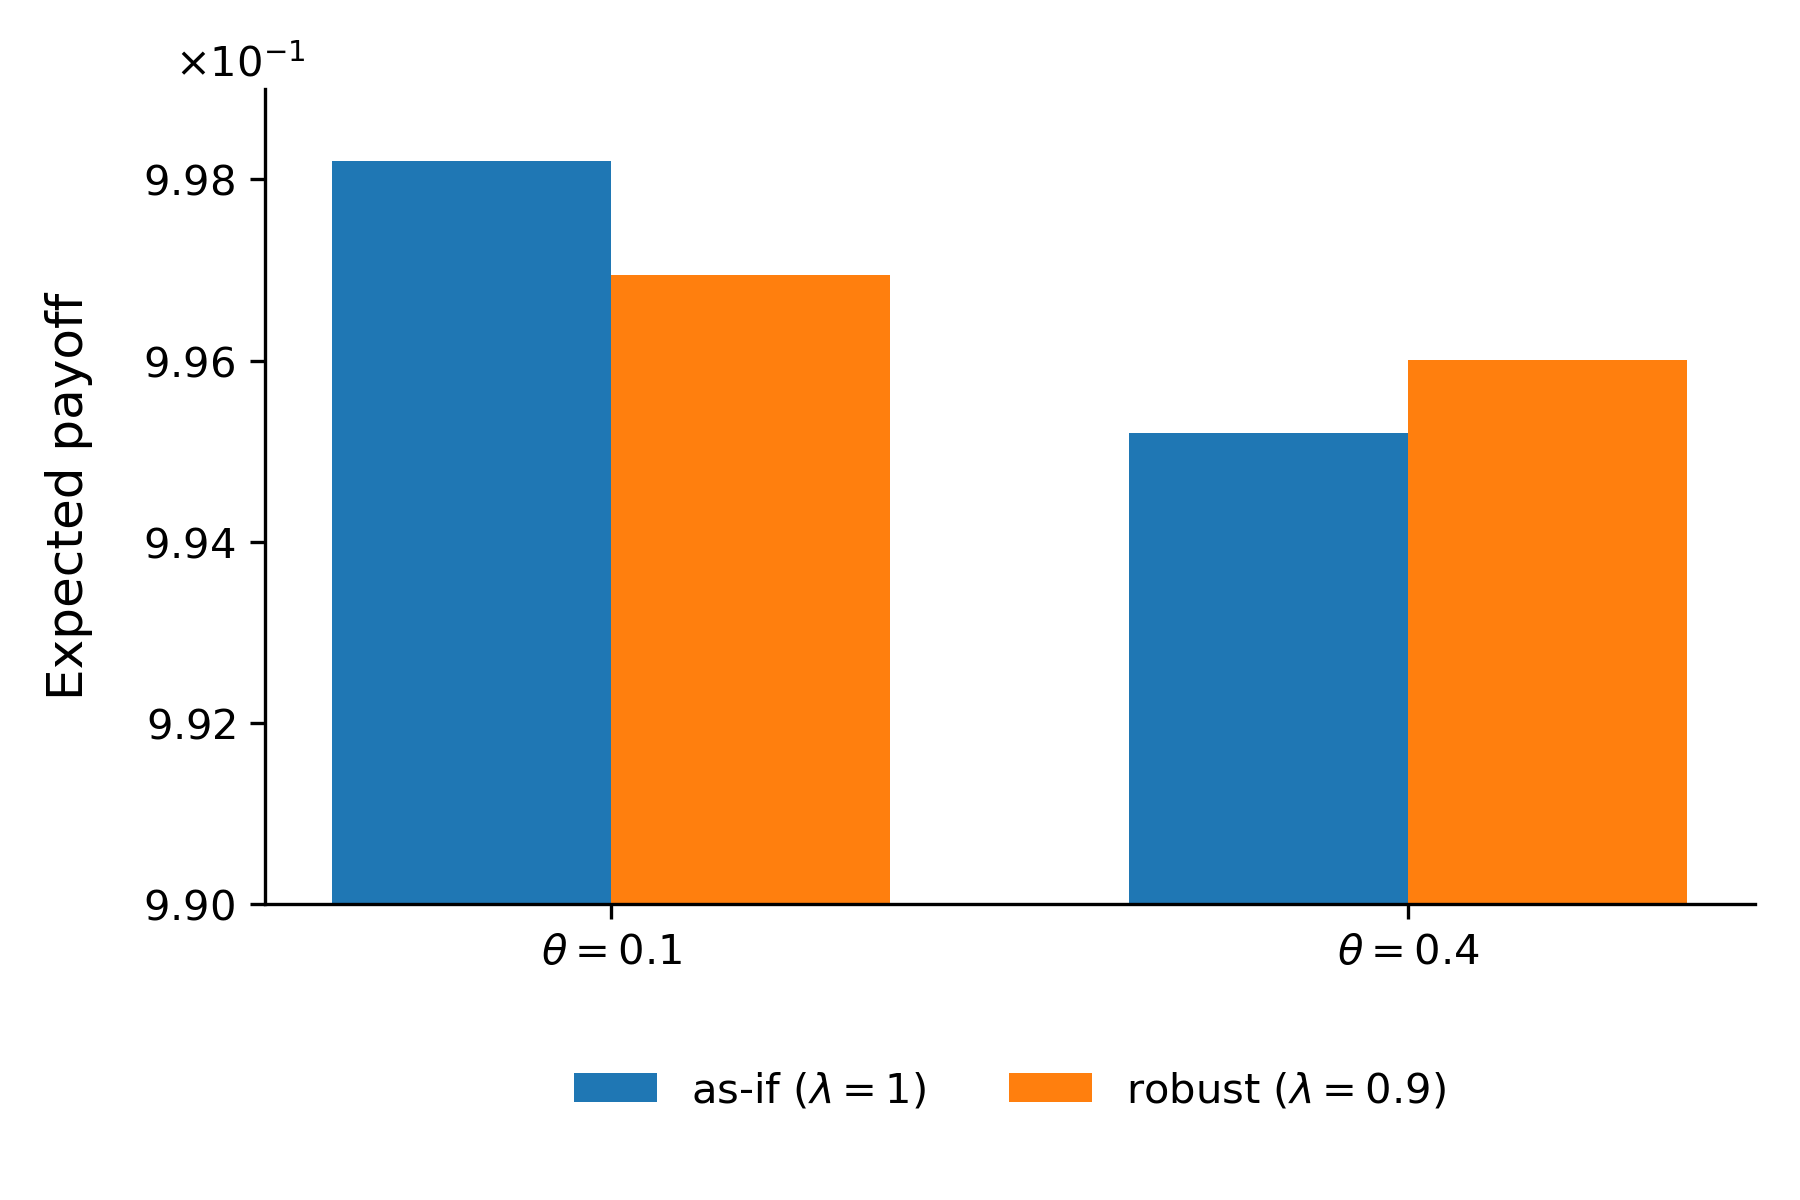
\includegraphics{fig-example-urn-exp-payoff-two-points}}}\hspace{0.3cm}
\subfloat[Performance]{\scalebox{0.50}{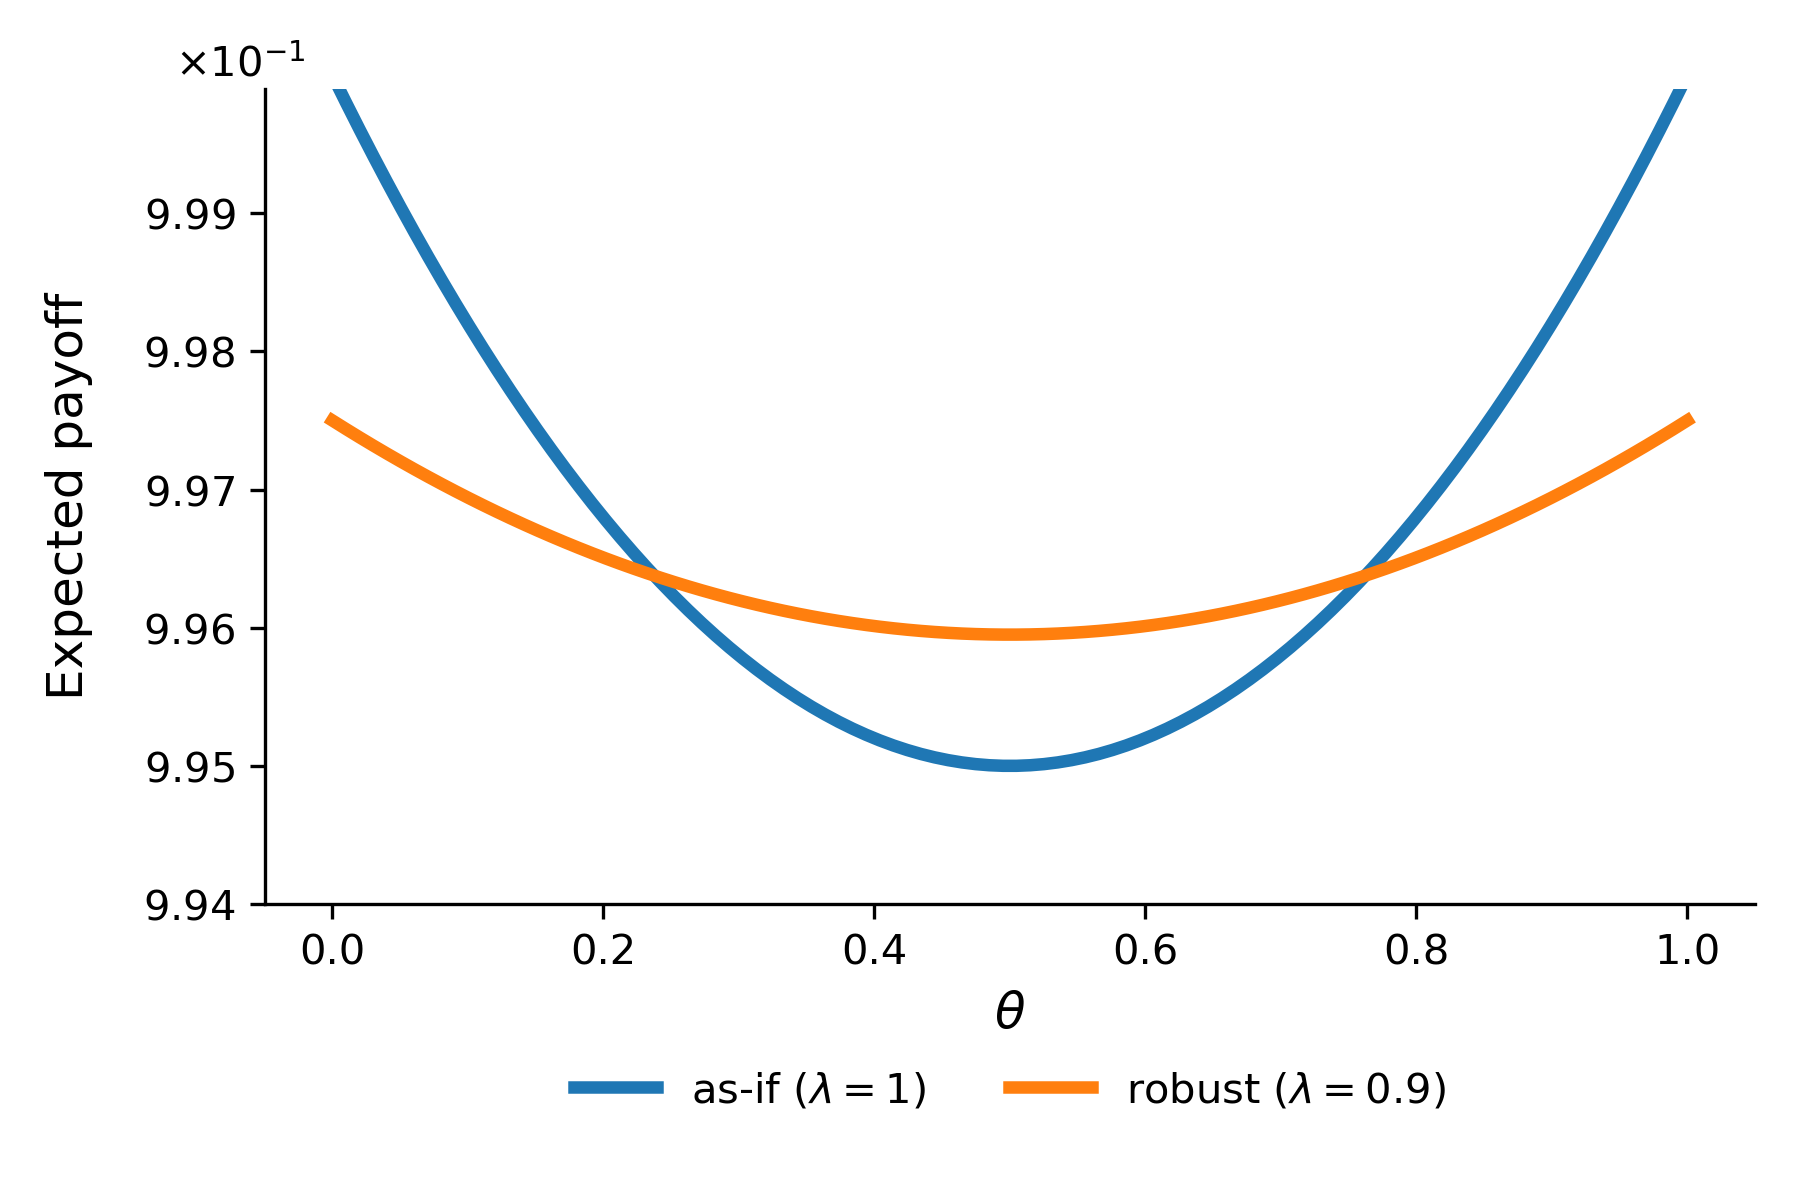
\includegraphics{fig-example-urn-payoff-functions}}}
\caption{Evaluating decision functions}\label{Measurement of performance}
\end{figure}\FloatBarrier

Figure \ref{Ranking of decision functions} ranks the two rules according to different decision-theoretic criteria. Both decision functions have their lowest expected payoff at $\theta = 0.5$. As the robust rule outperforms the as-if alternative at that point, the robust rule is preferred based on the maximin and minimax regret criteria. The maximin and minimax regret criteria are identical in this setting, as the payoff at the true proportion is constant across the parameter space.   Using the subjective Bayes criterion with a uniform prior, however, we select the as-if decision function as its better performance at the boundary of the parameter space is enough to offset its poor performance in the center.

\begin{figure}[h!]\centering
\scalebox{0.75}{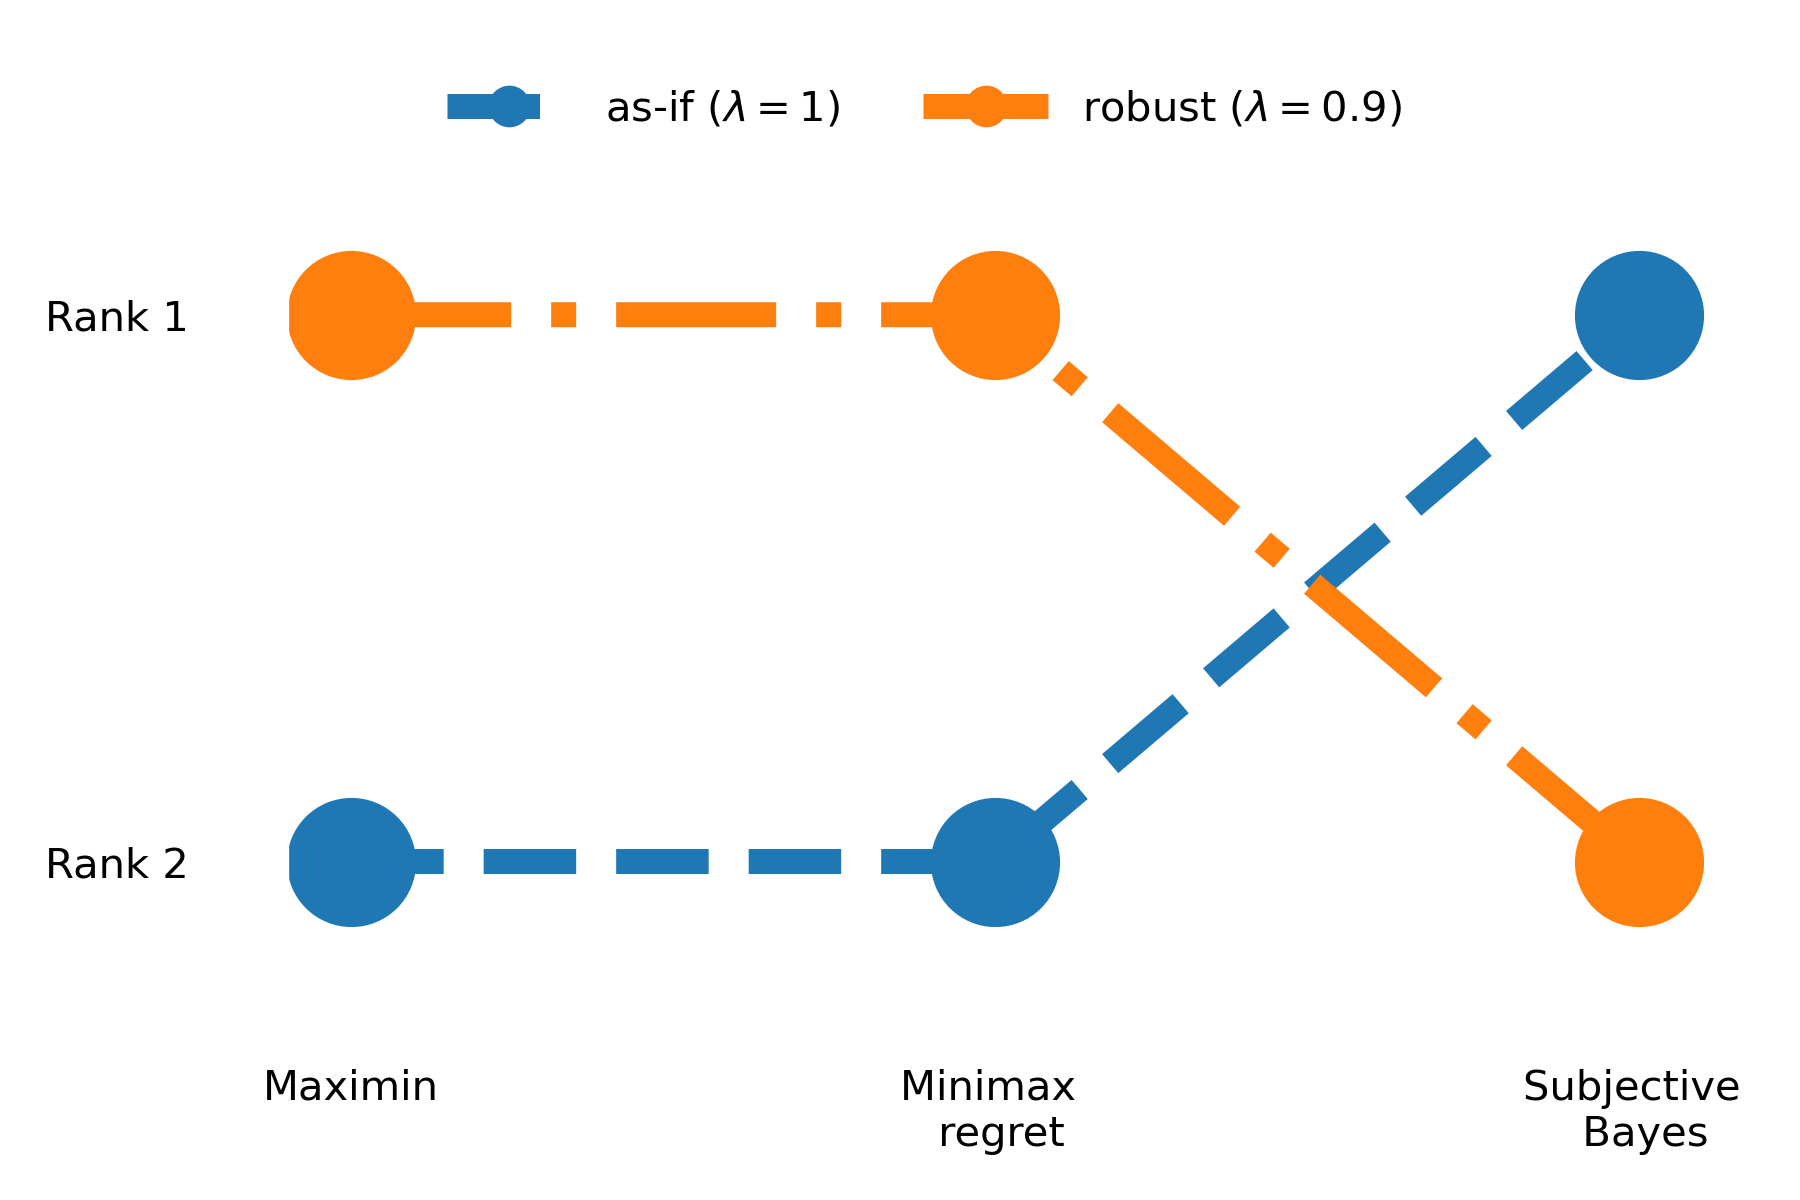
\includegraphics{fig-example-urn-ranks}}
\caption{Ranking of decision functions}\label{Ranking of decision functions}
\end{figure}\FloatBarrier

Returning to the whole set of decision functions, we can construct the optimal rule for the alternative criteria by varying $\lambda$ to maximize the relevant performance measure. For example, Figure \ref{Optimality of decision functions for urn} shows the optimal level of $\lambda$ for the maximin and subjective Bayes criterion.

\begin{figure}[h!]\centering
\scalebox{0.75}{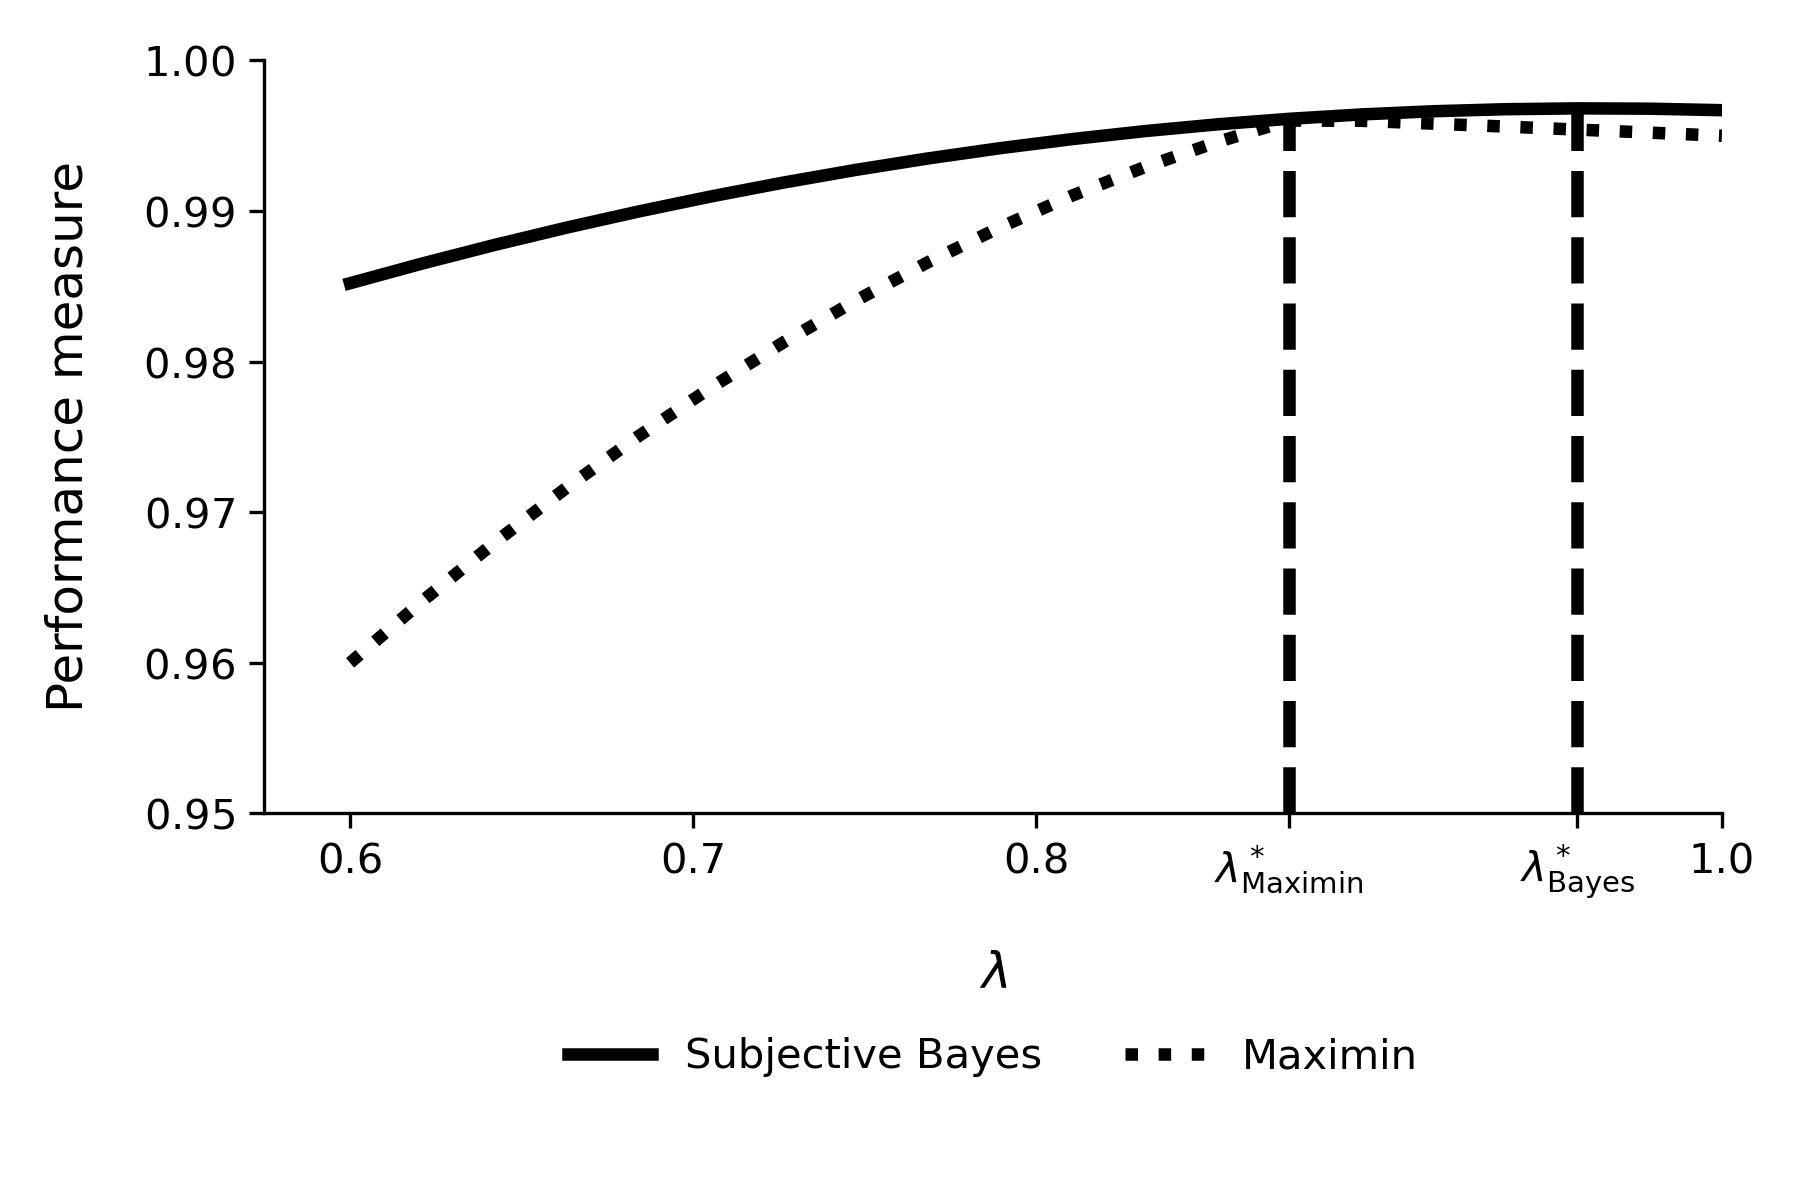
\includegraphics{fig-example-urn-optimal-sw}}\vspace{-0.9cm}
\begin{center}
\begin{minipage}[t]{0.5\columnwidth}
\item \scriptsize{\textbf{Notes:} We omit the performance measure for the minimax regret criterion as $\lambda^*_{\text{Maximin}} = \lambda^*_{\text{Regret}}$ in this setting as noted earlier.}
\end{minipage}
\end{center}
\caption{Optimality of decision functions}\label{Optimality of decision functions for urn}
\end{figure}\FloatBarrier

The as-if decision function $(\lambda=1.0)$ is not optimal under both criteria as at the optimum  $0.8 < \lambda^*_{\text{Maximin}} < \lambda^*_{\text{Bayes}} < 1$. The performance measure is more sensitive to the choice of $\lambda$ under the maximin criterion than subjective Bayes.\\

In summary, the urn example illustrates the performance comparison of alternative decision functions over the whole parameter space of a model, and it shows how to construct optimal decision functions within a set of rules for alternative decision-theoretic criteria. Next, we move to the more involved setting of a sequential dynamic decision problem with ambiguous transitions and explore a class of statistical decision functions frequently used in the operations research literature.
